\documentclass[a4paper,11pt,UTF8]{article}
\usepackage{ctex}
\usepackage{amsmath,amsthm,amssymb,amsfonts}
\usepackage{amsmath}
\usepackage[a4paper]{geometry}
\usepackage{graphicx}
\usepackage{microtype}
\usepackage{siunitx}
\usepackage{booktabs}
\usepackage[colorlinks=false, pdfborder={0 0 0}]{hyperref}
\usepackage{cleveref}
\usepackage{esint} 
\usepackage{graphicx}
\usepackage{ragged2e}
\usepackage{pifont}
\usepackage{extarrows}
\usepackage{mathptmx}
\usepackage{float}
\usepackage{caption}
\captionsetup[figure]{name={Figure}}
%opening
\title{Microelectronics Circuit Analysis and Design Homework(5th)}
\author{Yuejin Xie \quad U202210333}
\date{Sept 21st, 2023}
\begin{document}
\maketitle
\noindent3.27 The transistor in the circuit in Figure P3.27 has parameters $V_{T N} = 0.8 $V
and $K_n = 0.25$ mA/V$^2$. Sketch the load line and plot the $Q$-point for
(a) $V_{DD} = 4$V, $R_D=1k\Omega$ and (b) $V_{DD} = 5 $V, $R_D=3k\Omega$. What is the
operating bias region for each condition?\\
\begin{figure}[H] 
	\centering 
	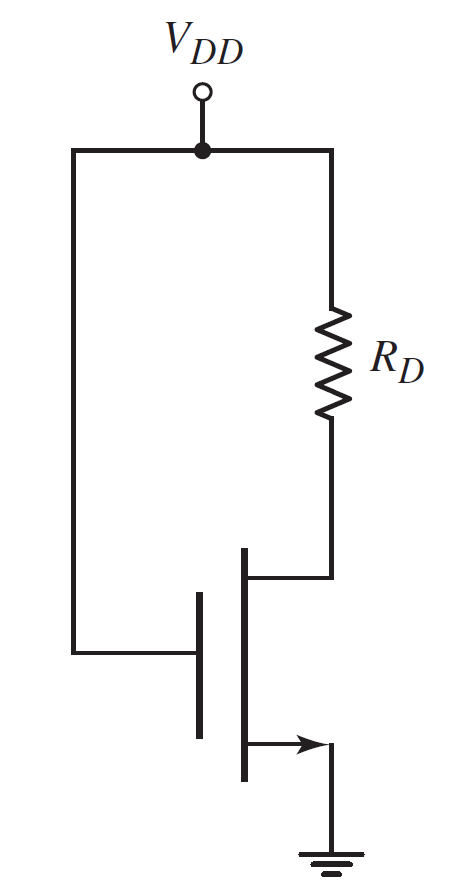
\includegraphics[scale=0.18]{MD3.27.png}
	\caption{Problem 3.27}
\end{figure}
\noindent Solution:\\
(a)Assume the transistor works in the saturation region:\\
$V_{GS}=V_{DD}=4V\Rightarrow i_{d}=K_n(V_{GS}-V_{TN})^2=2.56$mA.\\
$\therefore V_{DS}=V_{DD}-i_{d}R_{D}=1.44$V$<V_{GS}-V_{TN}\Rightarrow$ the transistor works in the nonsaturation region\\
$\therefore \begin{cases}
	i_{d}=K_n\left[2(V_{GS}-V_{TN})V_{DS}-V^2_{DS}\right]\\
	V_{DS}=V_{DD}-i_{d}R_{D}
\end{cases}\Rightarrow
\begin{cases}
	i_{d}=2.12\text{mA}\\
	V_{DS}=1.88\text{V}
\end{cases}$\\
(b)Assume the transistor works in the saturation region:\\
$V_{GS}=V_{DD}=4V\Rightarrow i_{d}=K_n(V_{GS}-V_{TN})^2=4.41$mA.\\
$\therefore V_{DS}=V_{DD}-i_{d}R_{D}=-8.23$V$<V_{GS}-V_{TN}\Rightarrow$ the transistor works in the nonsaturation region:\\
$\therefore \begin{cases}
	i_{d}=K_n\left[2(V_{GS}-V_{TN})V_{DS}-V^2_{DS}\right]\\
	V_{DS}=V_{DD}-i_{d}R_{D}
\end{cases}\Rightarrow
\therefore \begin{cases}
	i_{d}=1.42\text{mA}\\
	V_{DS}=0.741\text{V} 
\end{cases}
$\\
\noindent3.35 For the transistor in the circuit in Figure P3.35, the parameters are
$V_{T N} = 0.4$ V, $k^{\prime}_n= 120\mu\text{A/V}^2$, and $W/L = 25$. Determine $V_{GS}$, $I_D$, and $V_{DS}$. Sketch the load line and plot the Q-point.
\begin{figure}[H] 
	\centering 
	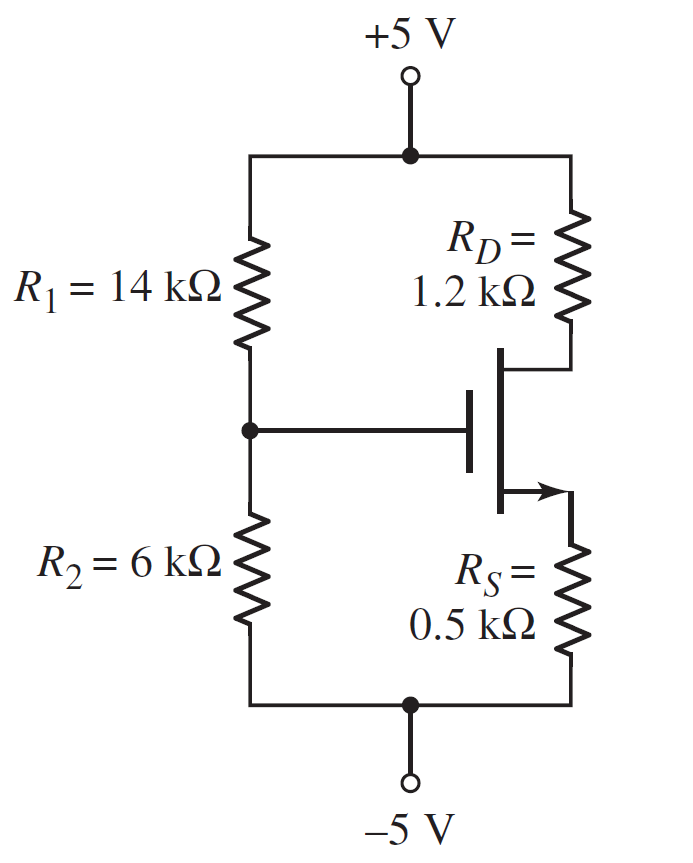
\includegraphics[scale=0.2]{MD3.35.png}
	\caption{Problem 3.35}
\end{figure}
\noindent Solution:\\
Actually, $\displaystyle K_n = \frac{k^\prime_n}{2}\cdot\frac{W}{L}=1.5\text{mA}/\text{V}^2$\\
Assume the transistor works in the saturation region:\\
$\displaystyle V_G=\frac{R_2}{R_1+R_2}(V_{DD}-V_{SS})+VSS=-2$V, $V_S=I_DR_S+V_{SS}=(0.5I_D-5) \text{V}$\\
$\therefore I_{D}=K_n(V_{G}-V_S-V_{TN})^2\Rightarrow I_D=2.58\text{mA}\text{ or }10.49\text{mA}(\text{Ignore})\\
\therefore V_{GS}=V_G-V_S=1.71\text{V}, V_{DS}=V_{DD}-I_DR_D- V_S=5.61\text{V}.
$

\end{document}